\documentclass[11pt, letterpaper]{report}
\input{../../homework.tex}
\usepackage{titlepageBU}
\title{Honors Differential Equations}
\date{10/23/24}
\courseID{MA 231}
\professor{Dr. Wayne}
\courseSection{A1}
\begin{document}
\makeproblem
\section*{Section 2.2 Problem 19}
(a,b,e)

\[
	\frac{\mathrm{d}x}{\mathrm{d}t} =v
.\]
\[
	\frac{\mathrm{d}v}{\mathrm{d}t} =-2v+3x-x^3
.\]
(a)
\begin{figure}[ht]
	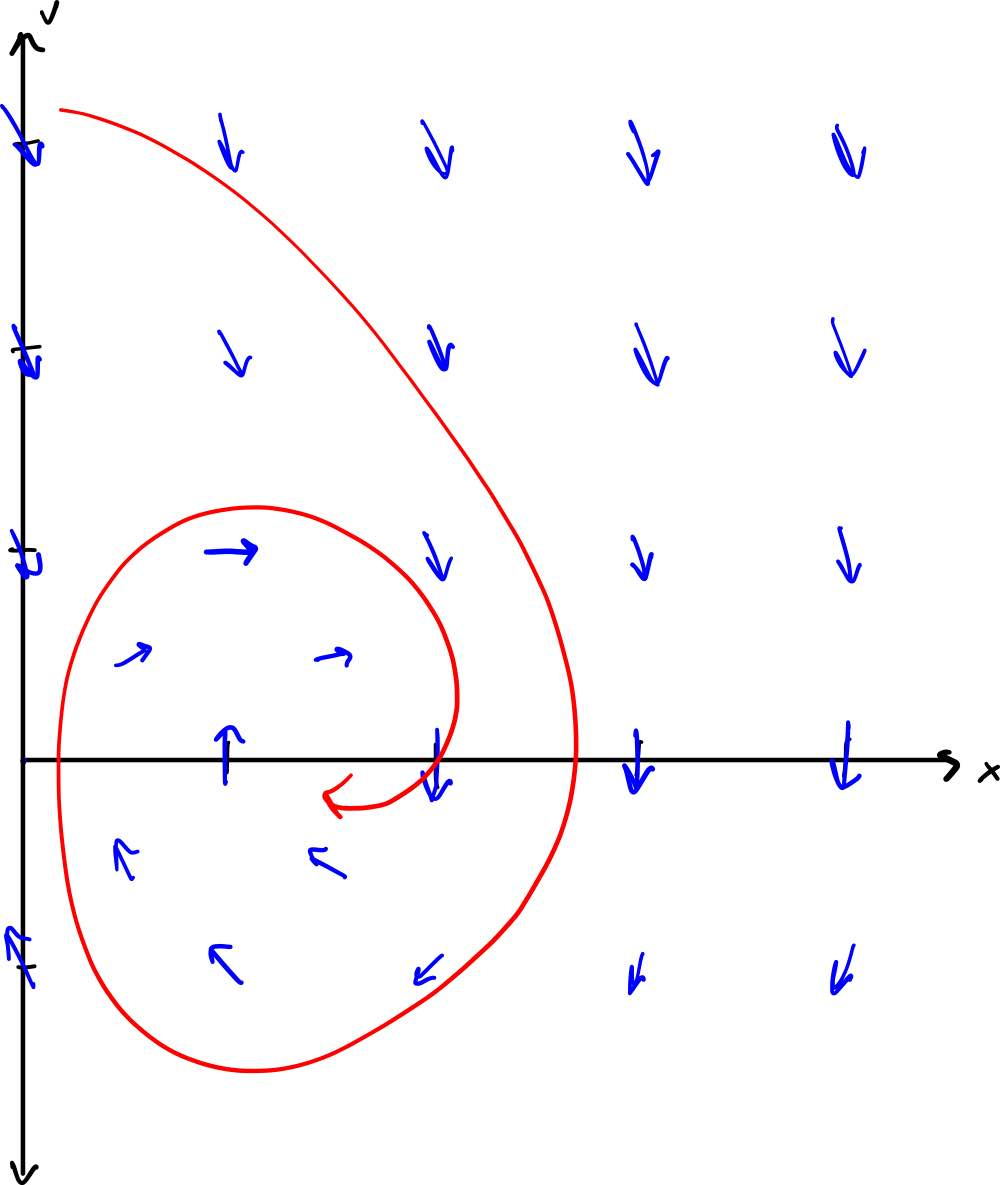
\includegraphics[scale=0.25]{vecs.jpg}
	\centering
\end{figure}

(b) Set $\frac{\mathrm{d}x}{\mathrm{d}t} ,\frac{\mathrm{d}^2x}{\mathrm{d}t^2} =0$. It follows that $v,\frac{\mathrm{d}v}{\mathrm{d}t} =0$. We thus have
\[
	x^3-3x=0
.\]
Note that I flipped the negative signs here. It follows that
\[
	x\left( x^2-3 \right) =0 \implies x\in \left\{ 0,\pm \sqrt{3}  \right\} 
.\]

(e) The solutions appear to spiral around the equilibrium points $\pm\sqrt{3} $ and $0$.There appears to be some level of overall tendency towards the equilibrium point $+\sqrt{3} $.

solns curl into the equilib it kinda goes down on positive thne up into
\section*{Section 2.4 Problem 13}
(a) Clearly,
\[
	y=y_0e^{-3t}
.\]
We then have
\[
	\frac{\mathrm{d}x}{\mathrm{d}t} =2x-8y_0^2e^{-6t}
.\]
We use the method of integrating factors.
\[
	\mu (t)=e^{\int -2 \,\mathrm{d} t}=e^{-2t}
.\]
\[
	x(t)=-e^{2t}\int e^{-2t}8y_0^2e^{-6t} \,\mathrm{d} t=-e^{2t}\int 8y_0^2e^{-8t} \,\mathrm{d} t=y_0^2e^{-6t}+x_0e^{2t}
.\]
Thus,
\[
	x(t)=x_0e^{2t}+y_0^2e^{-6t},\qquad y(t)=y_0e^{-3t}
.\]


(b) Let $\frac{\mathrm{d}x}{\mathrm{d}t} ,\frac{\mathrm{d}y}{\mathrm{d}t} =0$. We have $y=0$ trivially. It follows that $2x=0$, and thus $x=0$. Therefore, $(0,0)$ is the only equilibrium point.

(c) For $y_0=1$, we have
\[
	y(t)=e^{-3t}
.\]
For $x_0=0$, we have
\[
	x(t)=e^{-6t}
.\]
Note that we choose $t=0$ since Picard's theorem applies in the $xy$-plane, so the choice of $t$ is irrelevant.
\newpage
(eulers)
\begin{figure}[ht]
	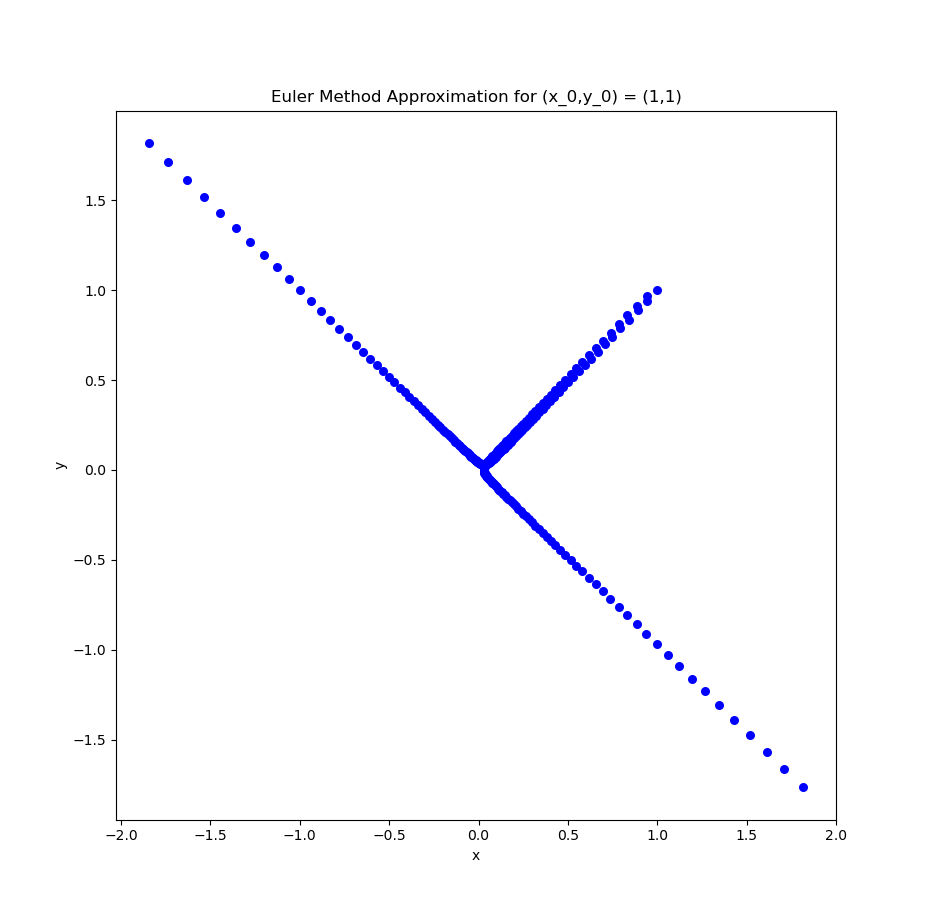
\includegraphics[scale=0.35]{xy11Euler.png}
	\centering
\end{figure}
\begin{figure}[ht]
	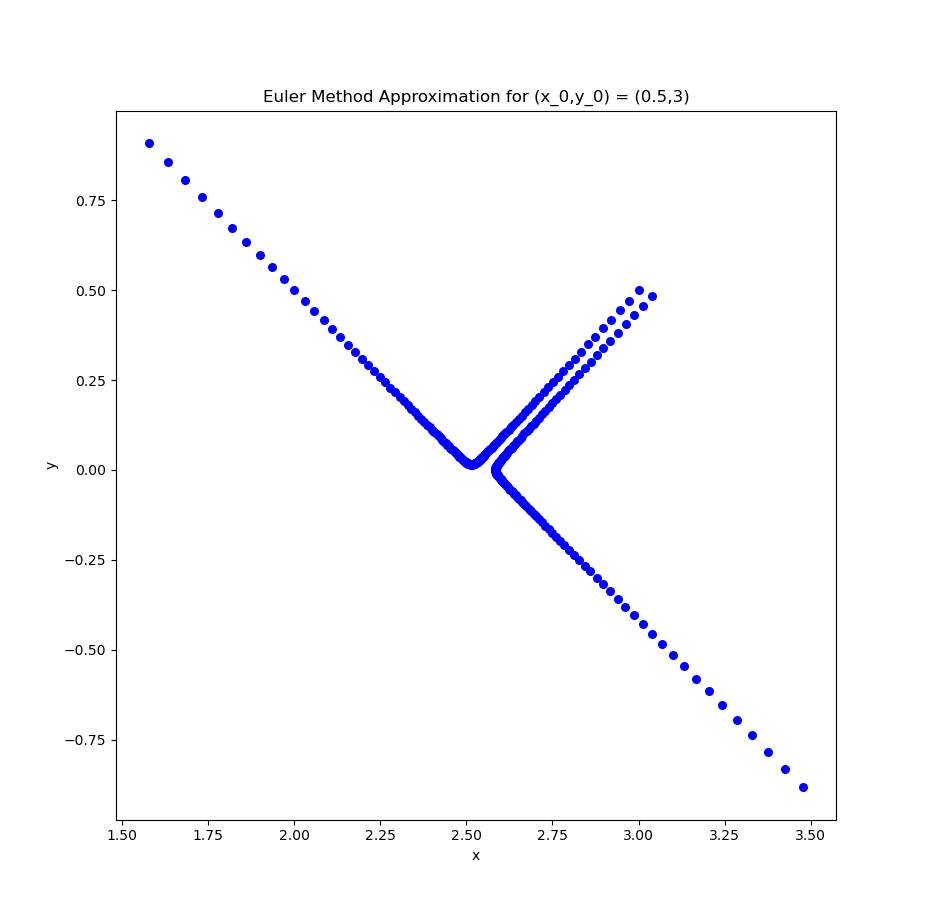
\includegraphics[scale=0.35]{xy053Euler.png}
	\centering
\end{figure}
\begin{figure}[ht]
	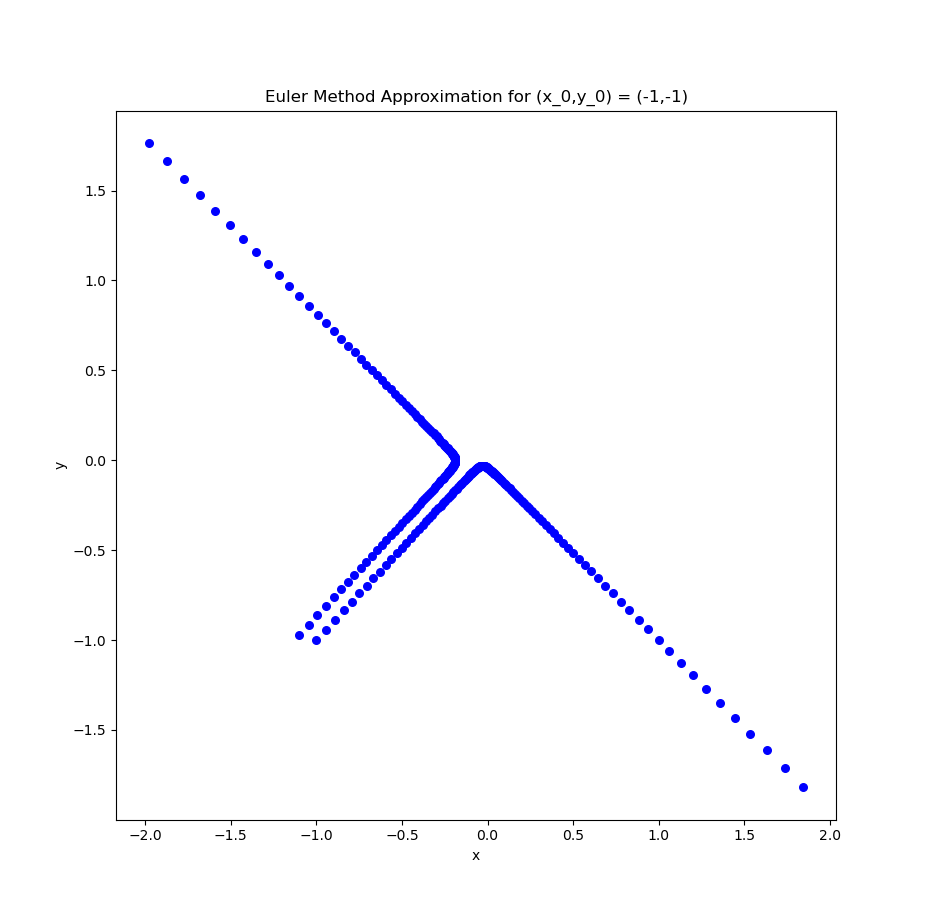
\includegraphics[scale=0.35]{xyn1n1Euler.png}
	\centering
\end{figure}
\newpage

\section*{Review 23}
True. You can see the solution curve passing through $(0,1)$ passes through $(0,0)$. Thus, taking $(1,0)$ to be the initial condition implies for some $t$, $(x,y)$ will equal $(0,0)$.
\section*{Review 24}
False. Picard's theorem applies, and the point $(1/2,0)$ is within the loop that goes from $(0,0)$ to $(1,0)$ and back. Thus, the graph must remain within this loop, and cannot tend to infinity.
\section*{Review 25}
True. Since they lie on the same line, they are the same equation.
\section*{Section 3.1 Problem 6}
\[
	\frac{\mathrm{d}\mathbf{Y}}{\mathrm{d}t} =\begin{bmatrix} 0&3 \\ -0.3&3\pi  \end{bmatrix} \mathbf{Y}(t)
.\]

\section*{Section 3.1 Problem 17}
(a) Define $v=\frac{\mathrm{d}y}{\mathrm{d}t} $. We have
\[
	\frac{\mathrm{d}v}{\mathrm{d}t} +pv+qy=0,\qquad \frac{\mathrm{d}y}{\mathrm{d}t} =v
.\]
Define $\mathbf{Y}(t)=(y,v)$. We have
\[
	\frac{\mathrm{d}\mathbf{Y}}{\mathrm{d}t} =\begin{bmatrix} 0&1 \\ -q&-p \end{bmatrix} \mathbf{Y}(t)
.\]
If $q=0$, we have
\[
	\frac{\mathrm{d}\mathbf{Y}}{\mathrm{d}t} =\begin{bmatrix} 0&1 \\ 0&-p \end{bmatrix} \begin{bmatrix} y \\ v \end{bmatrix} =v\begin{bmatrix} 1 \\ -p \end{bmatrix} 
.\]
It follows that
\[
	\frac{\mathrm{d}v}{\mathrm{d}t} =-pv \implies v=e^{-pt}
.\]
Additionally,
We do not need to find $y$ in terms of $t$, since if we substitute $\frac{\mathrm{d}\mathbf{Y}}{\mathrm{d}t} =\mathbf{0}$, we have
\[
	\mathbf{0}=v \begin{bmatrix} 1 \\ -p \end{bmatrix} 
.\]

Since the equation is no longer dependent on $y$, all values of $y$ are equilibria. This can be validated by setting $\frac{\mathrm{d}^2y}{\mathrm{d}t^2} ,\frac{\mathrm{d}t}{\mathrm{d}t} =0$ in the original equation:
\[
	qy=0
.\]
Since $q=0$, $y$ can be anything.

(b) Let $p,q=0$. We have
\[
	\mathbf{0}=\begin{bmatrix} 0&1 \\ 0&0 \end{bmatrix} \begin{bmatrix} y \\ v \end{bmatrix} \implies v=0
.\]
Since this equation does not depend on $y$ still, all points are equilibria. We can verify this using the original equation:
\[
	\frac{\mathrm{d}^2y}{\mathrm{d}t^2} =0
.\]
\section*{Section 3.1 Problem 24}
(a)
\[
	\frac{\mathrm{d}\mathbf{Y}_1}{\mathrm{d}t} =\frac{\mathrm{d}}{\mathrm{d}t} \begin{bmatrix} 0 \\ e^t \end{bmatrix} =\begin{bmatrix} 0 \\ e^t \end{bmatrix} 
.\]
\[
	\frac{\mathrm{d}\mathbf{Y}_1}{\mathrm{d}t} =\begin{bmatrix} 2&0 \\ 1&1 \end{bmatrix} \begin{bmatrix} 0 \\ e^t \end{bmatrix} =\begin{bmatrix} 0 \\ e^t \end{bmatrix} 
.\]
\[
	\frac{\mathrm{d}\mathbf{Y}_2}{\mathrm{d}t} =\frac{\mathrm{d}}{\mathrm{d}t} \begin{bmatrix} e^{2t} \\ e^{2t} \end{bmatrix} =\begin{bmatrix} 2e^{2t} \\ 2e^{2t} \end{bmatrix} 
.\]
\[
	\frac{\mathrm{d}\mathbf{Y}_2}{\mathrm{d}t} =\begin{bmatrix} 2&0 \\ 1&1 \end{bmatrix} \begin{bmatrix} e^{2t} \\ e^{2t} \end{bmatrix} =\begin{bmatrix} 2e^{2t} \\ e^{2t}+e^{2t} \end{bmatrix} 
.\]
(b) Every solution is a linear combination of our basis solutions $\mathbf{Y}_1(t),\mathbf{Y}_2(t)$, since they are linearly independent. Thus,
\[
	\mathbf{Y}(0)=c_1 \mathbf{Y}_1(t)+c_2 \mathbf{Y}_2(t)
.\]
We have
\[
	\begin{bmatrix} -2 \\ -1 \end{bmatrix} =\begin{bmatrix} 0 \\ c_1 \end{bmatrix} +\begin{bmatrix} c_2 \\ c_2 \end{bmatrix} \implies \begin{bmatrix} -2 \\ -1 \end{bmatrix} =\begin{bmatrix} c_2 \\ c_2+c_1 \end{bmatrix} 
.\]
We have $c_2=-2$, and thus $c_1=1$. Therefore,
\[
	\mathbf{Y}(t)=\mathbf{Y}_1(t)-2\mathbf{Y}_2(t)
.\]
\section*{Supplimental 1}
\begin{center}
	\[
		r=0.8\qquad\qquad\; r=2\qquad\qquad\; r=3.2
	\]
	\begin{tabular}{rr}
\toprule
$n$ & $z_n$ \\
\midrule
0 & 0.100000 \\
1 & 0.072000 \\
2 & 0.053453 \\
3 & 0.040476 \\
4 & 0.031071 \\
5 & 0.024084 \\
6 & 0.018803 \\
7 & 0.014760 \\
8 & 0.011634 \\
9 & 0.009199 \\
10 & 0.007291 \\
11 & 0.005790 \\
12 & 0.004605 \\
13 & 0.003667 \\
14 & 0.002923 \\
15 & 0.002332 \\
\bottomrule
\end{tabular}
\begin{tabular}{rr}
\toprule
$n$ & $z_n$ \\
\midrule
0 & 0.100000 \\
1 & 0.180000 \\
2 & 0.295200 \\
3 & 0.416114 \\
4 & 0.485926 \\
5 & 0.499604 \\
6 & 0.500000 \\
7 & 0.500000 \\
8 & 0.500000 \\
9 & 0.500000 \\
10 & 0.500000 \\
11 & 0.500000 \\
12 & 0.500000 \\
13 & 0.500000 \\
14 & 0.500000 \\
15 & 0.500000 \\
\bottomrule
\end{tabular}
\begin{tabular}{rr}
\toprule
$n$ & $z_n$ \\
\midrule
0 & 0.100000 \\
1 & 0.288000 \\
2 & 0.656179 \\
3 & 0.721946 \\
4 & 0.642368 \\
5 & 0.735140 \\
6 & 0.623069 \\
7 & 0.751533 \\
8 & 0.597540 \\
9 & 0.769555 \\
10 & 0.567488 \\
11 & 0.785425 \\
12 & 0.539304 \\
13 & 0.795057 \\
14 & 0.521413 \\
15 & 0.798533 \\
\bottomrule
\end{tabular}
\end{center}
For $r=0.8$, we notice that $z_n$ appears to be asymptotically approaching $0$. It appears as though $0$ is an equilibrium point.

For $r=2$, notice that $z_n$ rapidly approaches $0.5$ and stabilizes there. Clearly, $0.5$ is an equilibrium point. In the continuous case, $z_n$ would not actually reach $0.5$, and it's possible it actually hasn't reached it and there are simply too many decimals for my code to handle. However, it's possible that since the system is discrete, it is allowed to reach and stabilize at the equilibrium point in finite time. It appears to approach it fairly linearly, as compared to asymptotically in the case of $r=0.8$.

For $r=3.2$, we notice that it rapidly approaches $0.65$, but then slows down and begins to oscilate between $0.6$ish and $0.7$ish It appears to be oscillating around an equilibrium point. The most interesting part is that the oscillations appear to be \emph{increasing} in amplitude, as compared to a general continuous case, where they usually decrease. Notice how they start around $0.72$ and $0.65$, decrease slightly, then go up to $0.79$ and $0.52$, which is a significantly larger delta. This is unlike the behaviour of any of the previous solutions.

I was so curious about the case for $r=3.2$ that I ran the code for larger values of $n$.

\begin{center}
\begin{tabular}{rr}
\toprule
$n$ & $z_n$ \\
\midrule
0 & 0.100000 \\
1 & 0.288000 \\
2 & 0.656179 \\
3 & 0.721946 \\
4 & 0.642368 \\
5 & 0.735140 \\
6 & 0.623069 \\
7 & 0.751533 \\
8 & 0.597540 \\
9 & 0.769555 \\
10 & 0.567488 \\
11 & 0.785425 \\
12 & 0.539304 \\
13 & 0.795057 \\
14 & 0.521413 \\
15 & 0.798533 \\
16 & 0.514810 \\
17 & 0.799298 \\
18 & 0.513346 \\
19 & 0.799430 \\
20 & 0.513093 \\
21 & 0.799451 \\
22 & 0.513052 \\
23 & 0.799455 \\
24 & 0.513046 \\
25 & 0.799455 \\
26 & 0.513045 \\
27 & 0.799455 \\
28 & 0.513045 \\
29 & 0.799455 \\
30 & 0.513045 \\
\bottomrule
\end{tabular}
\end{center}
It appears to stabilize at two different points; instead of approaching a single equilibria, it oscillates between two different points. I hope we learn more about this behavior, because this is very interesting.
\end{document}
